\chapter{Introduction}
\emph{The chapter starts with a background describing why road condition monitoring is important and who Trafikverket are, how road condition data is collected today and why the technology behind it needs improvement. An objective for the project is defined followed by its delimitations. Lastly, a thesis structure is presented to simplify navigation through different parts of the project.}

\section{Background}
	Living in cold areas of the world usually means work for invididual people, municipalities and companies in trying to maintain a non-winter-like infrastructure. This of course, also involves winter road maintenance. Salting and plowing roads is an investment in not only saving lives, but also in lowering socio-economic costs: In two scenarios on a road with 2 cm snow and a daily traffic flow of 2000 vehicles, one with a salted and ploughed road taking four hours to drive, and another scenario on the same road without winter maintenance taking five hours to drive. The total socio-economic costs are 3.5\% higher in the non-maintained road, mainly due to increased travel time and thus higher accident costs \cite{ARTICLE:1}. 

	Despite the socio-economic savings in performing winter road maintenance, it still represents a notable economic cost. Trafikverket, the agency in charge of road state road maintenance in Sweden, reported that winter road maintenance were roughly 18\% of the total road maintenance costs in 2013 \cite{REPORT:1}. Local contracters are hired to carry out the plowing and salting of state roads, with requirements on both ends regarding when to plow, which roads to prioritize etc. Trafikverket has over 800 Road Weather Information Systems (RWIS)(Fig. \ref{img:rwis}) distributed across state roads in Sweden which are used by contracters to carry out winter road maintenance work. 
\begin{figure}[H]
	\centering
	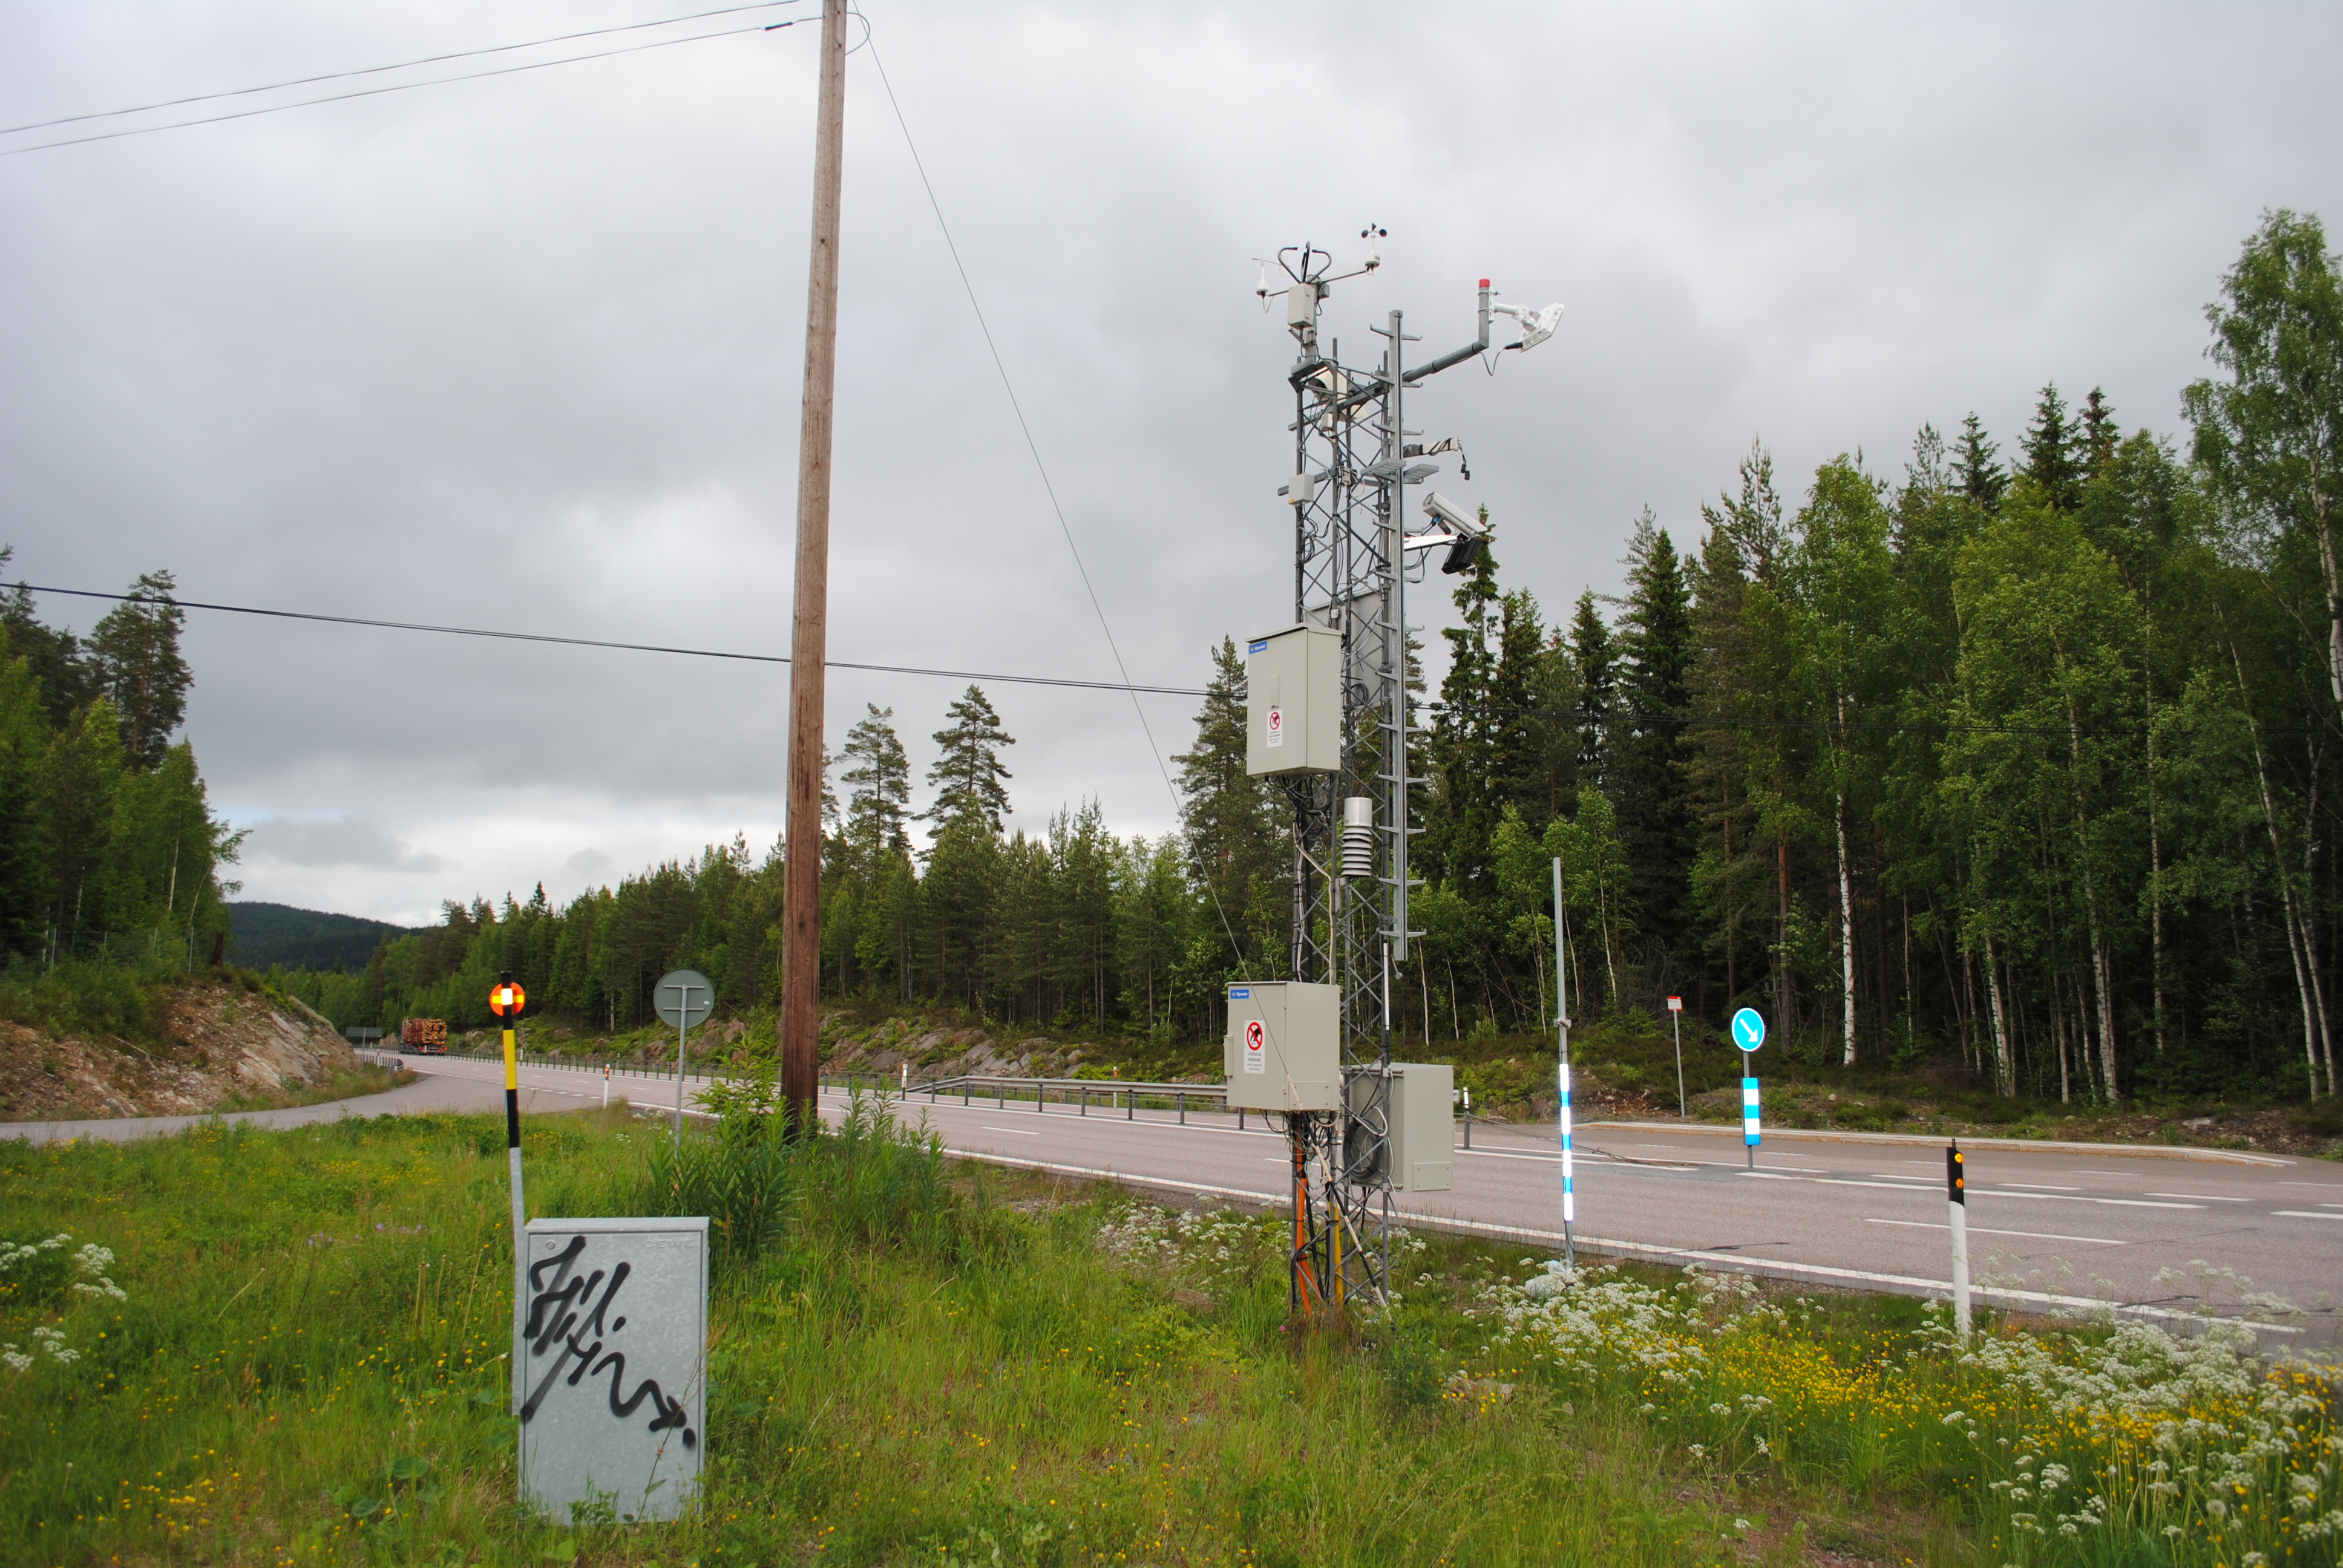
\includegraphics[width=0.8\textwidth]{media/Rwis_station_Myggsjon_01.JPG}
	\caption{RWIS Station at sensor site Myggsjön \cite{IMAGE:1}.}
	\label{img:rwis}
\end{figure}
Table 
\begin{tabular}[3]{c | c | c}
    	Operation & worst-case cost & time complexity \\
    	\hline
    	Insert $x$ into $l_i$ & 2 & $O(1)$  \\
   	Update $count_i$ & 1 &$O(1)$ \\
	\label{table:rwis}
\end{tabular}
asdasd
%\begin{itemize}
	%Why improve road condition monitoring?
	%what is Trafikverket and what do they do? 
	%weatherstations, what are they? What's the road surface temperature sensor?
	%why is it desirable to simulate the road sensor?
	%what is machine learning? \cite{WEBSITE:1}

%\end{itemize}

\section{Objective}
	The objective is to determine if a road surface temperature sensor can be simulated with prediction models based on historic data from road weather information systems.
\section{Delimitations}

\section{Thesis structure}
